\documentclass[11pt]{article}
\usepackage[spanish,es-tabla,es-nodecimaldot,es-noshorthands]{babel}
\usepackage[utf8]{inputenc}
\usepackage[T1]{fontenc}
\usepackage{lmodern}
\usepackage[margin=2.5cm]{geometry}
\usepackage{amsmath}
\usepackage{graphicx}
\usepackage{booktabs}
\usepackage{tabularx}
\usepackage{longtable}
\usepackage{float}
\usepackage{enumitem}
\usepackage{tikz}
\usetikzlibrary{arrows.meta, positioning, calc, babel}
\usepackage[hidelinks]{hyperref}

\setlist{itemsep=2pt, topsep=4pt}

\tikzset{
  box/.style    = {draw=black!75, semithick, rounded corners=1.5pt, align=center,
                   minimum height=1.1cm, minimum width=2.6cm, font=\footnotesize,
                   fill=white},
  shade/.style  = {box, fill=black!7},
  sig/.style    = {-{Stealth[length=2mm]}, semithick},
  cell/.style   = {draw=black!75, minimum height=0.55cm, minimum width=1.1cm,
                   font=\scriptsize\ttfamily, inner sep=1pt, anchor=south west},
  lab/.style    = {font=\scriptsize, midway, above},
  note/.style   = {font=\scriptsize\itshape, align=center},
  rowlab/.style = {font=\footnotesize, anchor=east},
}

\newcommand{\code}[1]{\texttt{#1}}
\newcommand{\us}{\,$\mu$s}

\title{Informe técnico de avance\\[2pt]
       \large Implementación y validación del enlace USB--SPI full-duplex\\
       de la DAQ basada en dsPIC33CK64MC105}
\author{Haniel Ulises\\Servicio social}
\date{6 de octubre de 2026}

\begin{document}
\maketitle

\begin{abstract}
Se informa el trabajo realizado entre el 1 y el 6 de octubre de 2026 para
sustituir el protocolo de comunicación entre Simulink y la tarjeta de
adquisición basada en el microcontrolador dsPIC33CK64MC105 y el puente
USB--SPI FT2232H. Se implementó el esquema planteado en la propuesta: una
transferencia full-duplex de ocho bytes por paso de simulación, delimitada
por la señal de selección de esclavo, protegida con número de secuencia y
CRC-8, y atendida en el dsPIC por el controlador DMA. Se desarrollaron,
además, un programa de prueba del enlace para Windows y Linux, un visor en
tiempo real, un generador de reportes y una batería de pruebas automatizada.
Las campañas de prueba sobre la tarjeta permitieron identificar y corregir
dos causas de error sucesivas. Con el reloj de 4\,MHz, la latencia del SPI
esclavo y la duración de la interrupción de fin de trama dañaban la mayoría
de las respuestas; ambos efectos se eliminaron al activar el PLL
($F_{cy} = 50$\,MHz). Quedó una tasa residual de entre 0.025\,\% y 1\,\%
de transferencias dañadas, cuyo origen se determinó como pulsos falsos en la
señal \code{CS} causados por la ausencia de una tierra común entre las
tarjetas. Con un cable de GND entre
la Curiosity Nano y el FT2232H, las cuatro pruebas de 100\,000 tramas
concluyeron sin errores. La salida analógica respondió a una rampa de
$\pm 1$\,V sin errores de comunicación; queda pendiente su verificación con
osciloscopio, la conexión del motor y del encoder, y la validación del
bloque de Simulink.
\end{abstract}

\tableofcontents
\newpage

% ===========================================================================
\section{Introducción}

\subsection{Antecedentes}

El sistema DAQ-SPI emula una tarjeta de adquisición de datos para el control
de un motor de corriente directa desde Simulink. La PC se comunica por USB con
un FT2232H que opera como maestro SPI; el dsPIC33CK64MC105, montado en una
tarjeta Curiosity Nano, actúa como esclavo, escribe la salida analógica en un
DAC8554 y cuenta los pulsos del encoder con su módulo QEI.

En la versión anterior, la escritura al DAC y la lectura del encoder se
realizaban con dos transacciones independientes (\code{SPI\_Write} y
\code{SPI\_Read}) desde tres S-Functions. Como se documentó en la propuesta
(\code{docs/propuesta.pdf}), ese esquema utilizaba el bus como un canal
half-duplex: cada transacción introducía o descartaba bytes que el otro
extremo no esperaba, las FIFOs de cuatro niveles del SPI esclavo se
desbordaban, la bandera \code{SPIROV} detenía la recepción de forma
permanente y la trama no se delimitaba con \code{CS}. Además, al terminar la
simulación se enviaba el código \code{0x0000}, que corresponde a $-2.5$\,V, de
modo que el motor quedaba energizado.

\subsection{Objetivos}

\begin{enumerate}
\item Implementar el protocolo propuesto: una sola transferencia full-duplex
  de longitud fija por paso de simulación, con detección de errores.
\item Reescribir el firmware del dsPIC para que el movimiento de datos del SPI
  no dependa de la CPU.
\item Disponer de herramientas que permitan medir el enlace sin Simulink,
  con un criterio de aceptación de cero errores en al menos 100\,000 tramas.
\item Sustituir las tres S-Functions por un solo bloque de Simulink.
\item Validar la salida analógica y la lectura del encoder con el motor.
\end{enumerate}

\subsection{Estado general}

La tabla~\ref{tab:etapas} resume el avance respecto al plan de validación de
la propuesta.

\begin{table}[H]
\centering
\small
\begin{tabularx}{\linewidth}{@{}lXl@{}}
\toprule
Etapa & Alcance & Estado \\
\midrule
1. Firmware & \code{dsPicDaq}: SPI1 con DMA, PLL, vigilancia, causa de reinicio & Concluida \\
2. Prueba del enlace & \code{prueba\_enlace}, visor, reportes; 100\,000 tramas sin errores & Concluida \\
3. Salida analógica & Rampa de $\pm1$\,V enviada sin errores; falta osciloscopio & En curso \\
4. Simulink & S-Function \code{daqPic} escrita; falta compilarla y probarla en Windows & Pendiente \\
5. Pruebas con el motor & Motor y encoder identificados; falta etapa de potencia & Pendiente \\
\bottomrule
\end{tabularx}
\caption{Estado de las etapas al 6 de octubre de 2026.}
\label{tab:etapas}
\end{table}

% ===========================================================================
\section{Descripción del sistema implementado}

\subsection{Componentes}

\begin{itemize}
\item \textbf{PC.} Windows 11 con MATLAB/Simulink para la operación, y Linux
  (Fedora 43) para el desarrollo y las pruebas del enlace.
\item \textbf{Puente USB--SPI.} FT2232H, canal A en modo MPSSE, maestro SPI en
  modo~0 a 1\,MHz, con \code{CS} activo en bajo en \code{ADBUS3}. Su EEPROM
  está reprogramada con el identificador \code{2099:0001} (``Custom DAC USB
  Bridge'', CINVESTAV).
\item \textbf{Microcontrolador.} dsPIC33CK64MC105 en la tarjeta Curiosity
  Nano, con depurador nEDBG y programación por arrastre a la unidad
  \code{CURIOSITY}.
\item \textbf{Convertidor digital-analógico.} DAC8554 de Texas Instruments
  (cuatro canales, 16 bits), en encapsulado TSSOP-16 montado sobre un
  adaptador Proto-Advantage PA0017C. Se utiliza el canal A (\code{VOUTA},
  terminal~1).
\item \textbf{Planta.} Motorreductor Pittman GM8724S017-R1 de 14\,V con
  encoder incremental de 500 ciclos por revolución.
\end{itemize}

\subsection{Conexiones}

La tabla~\ref{tab:conexiones} reproduce las conexiones vigentes. La última
fila, el cable de tierra entre las tarjetas, se agregó como resultado de este
trabajo (sección~\ref{sec:cs}).

\begin{table}[H]
\centering
\small
\begin{tabular}{@{}llll@{}}
\toprule
Señal & dsPIC & FT2232H & DAC8554 \\
\midrule
SCK1 (entrada) & RB13 & AD0 (SCK) & \\
SDI1 & RB14 & AD1 (MOSI) & \\
SDO1 & RB11 & AD2 (MISO) & \\
SS1 / INT1 & RB10 & AD3 (\code{CS}) & \\
SCK2 & RB0 & & terminal 10 (SCLK) \\
SDO2 & RB2 & & terminal 11 (DIN) \\
SYNC (GPIO) & RB4 & & terminal 9 (SYNC) \\
QEI A / B & RB8 / RB9 & & \\
LED0 & RD10 & & \\
GND & GND (junto a RB10) & GND & terminal 6 (GND) \\
\bottomrule
\end{tabular}
\caption{Conexiones del sistema.}
\label{tab:conexiones}
\end{table}

\subsection{Protocolo de comunicación}

Cada paso de simulación ejecuta una transferencia de ocho bytes en ambas
direcciones (tabla~\ref{tab:trama}). La respuesta que el dsPIC envía en la
transferencia $k$ se construyó al terminar la transferencia $k-1$; por ello
el byte~1 de la respuesta es el eco del número de secuencia de la última
trama válida recibida, lo que permite a la PC detectar tramas perdidas. El
CRC-8 utiliza el polinomio \code{0x07} (CRC-8/SMBUS) y se calcula por tabla.
El formato, las constantes y la conversión de voltaje a código se definen en
un solo archivo, \code{protocolo/daq\_protocolo.h}, que comparten el firmware
y todos los programas de la PC.

\begin{table}[H]
\centering
\small
\begin{tabular}{@{}cll|ll@{}}
\toprule
Byte & \multicolumn{2}{l|}{PC $\to$ dsPIC (MOSI)} & \multicolumn{2}{l}{dsPIC $\to$ PC (MISO)} \\ \midrule
0   & \code{0xA5}   & inicio de trama              & \code{0x5A}   & inicio de trama \\
1   & \code{seq}    & número de secuencia          & \code{seq}    & eco de la última trama válida \\
2   & \code{dac\_h} & valor del DAC, byte alto     & \code{enc0}   & posición del encoder \\
3   & \code{dac\_l} & valor del DAC, byte bajo     & \code{enc1}   & (entero de 32 bits \\
4   & \code{flags}  & banderas de control          & \code{enc2}   & con signo, \\
5   & ---           & reservado                    & \code{enc3}   & \emph{little-endian}) \\
6   & ---           & reservado                    & \code{status} & estado del dsPIC \\
7   & \code{crc}    & CRC-8 de los bytes 0 a 6     & \code{crc}    & CRC-8 de los bytes 0 a 6 \\
\bottomrule
\end{tabular}
\caption{Formato de trama.}
\label{tab:trama}
\end{table}

El valor del DAC se obtiene como $\text{código} = 13107\,(V + 2.5)$, con
saturación a $\pm2.5$\,V; un valor no numérico se lleva a 0\,V. El código
32\,767 corresponde a 0\,V. El byte \code{flags} habilita la salida
analógica (bit~0; con cero el DAC se lleva a 0\,V) y ordena poner en cero el
contador del encoder (bit~1). El byte \code{status} se describe en la
tabla~\ref{tab:status}; los cuatro bits altos se agregaron durante este
trabajo para reportar la causa del último reinicio del dsPIC.

\begin{table}[H]
\centering
\small
\begin{tabularx}{\linewidth}{@{}llX@{}}
\toprule
Bits & Nombre & Significado \\
\midrule
0 & \code{ERR\_CRC} & la última trama recibida tuvo CRC incorrecto \\
1 & \code{ERR\_INICIO} & la última trama recibida no comenzó con \code{0xA5} \\
2 & \code{VIGILANCIA} & transcurrieron 50\,ms sin una trama válida; el DAC se llevó a 0\,V \\
3 & \code{ERR\_LONGITUD} & la última transferencia no tuvo exactamente ocho bytes \\
4--7 & \code{REINICIO} & causa del arranque (encendido, bajo voltaje, MCLR, watchdog, software, opcode ilegal, configuración o alguna de las trampas); se envía una sola vez, en la primera respuesta después del arranque \\
\bottomrule
\end{tabularx}
\caption{Campos del byte \code{status}.}
\label{tab:status}
\end{table}

% ===========================================================================
\section{Firmware \code{dsPicDaq}}

El firmware se escribió a partir del proyecto anterior
\code{dsPicController}, cuya configuración generada por MCC se conserva
para los pines y periféricos que no cambian. Se encuentra en
\code{MPLAB/dsPicDaq.X} y su imagen compilada en \code{MPLAB/dsPicDaq.hex}.

\subsection{Enlace SPI con DMA}

SPI1 opera como esclavo en modo~0 (\code{CKP} = 0, \code{CKE} = 1), con la
entrada de selección \code{SS1} habilitada y en modo de buffer estándar. La
FIFO del modo mejorado, de cuatro niveles en 8 bits, no alcanza para una
trama, por lo que no aporta en este esquema. Dos canales del controlador DMA
atienden el módulo:

\begin{itemize}
\item \textbf{DMA0} (disparo \code{0x02}, SPI1 RX): copia \code{SPI1BUFL} a
  \code{rx\_dma[]} con cada byte recibido.
\item \textbf{DMA1} (disparo \code{0x03}, SPI1 TX): copia \code{tx\_dma[1..7]}
  a \code{SPI1BUFL} cada vez que el buffer de transmisión queda vacío. El
  primer byte se escribe directamente al armar la trama.
\end{itemize}

Los eventos de SPI1 se usan sólo como disparo del DMA; las interrupciones de
CPU del módulo permanecen deshabilitadas. Durante la transferencia la CPU no
interviene.

\subsection{Fin de trama}

\code{CS} (RB10) se lleva también a la entrada INT1 mediante PPS. La
interrupción, configurada en el flanco de subida, ejecuta la secuencia
siguiente:

\begin{enumerate}
\item Deshabilita ambos canales de DMA.
\item Valida la trama: el canal de RX debe haber terminado, el buffer de
  recepción debe estar vacío y sin desbordamiento (exactamente ocho bytes);
  después se revisan el encabezado y el CRC. Una trama válida actualiza el
  valor del DAC, el eco de secuencia y reinicia la vigilancia.
\item Reinicia SPI1 deshabilitándolo y habilitándolo, lo que vacía los
  buffers y borra \code{SPIROV}, de modo que cada trama comienza alineada.
\item Lee el contador del QEI y construye la respuesta siguiente.
\item Programa de nuevo los dos canales de DMA.
\end{enumerate}

La terminal RD10 permanece en alto mientras se ejecuta la rutina, lo que
permite medir su duración con un analizador lógico.

\subsection{Vigilancia}

Timer1 genera una interrupción cada 50\,ms; cada trama válida lo reinicia.
Si expira, el DAC se lleva a 0\,V y se reporta la bandera \code{VIGILANCIA}
una sola vez. Sólo una trama válida restablece la operación. Con esto, si
Simulink se detiene o la PC deja de enviar tramas, el motor se desenergiza.

\subsection{Reloj del sistema}

Los firmwares anteriores operaban sin PLL ($F_{osc} = 8$\,MHz,
$F_{cy} = 4$\,MHz). Las primeras pruebas mostraron que ese reloj era
insuficiente (sección~\ref{sec:4mhz}), por lo que \code{reloj.c} configura el
oscilador FRC de 8\,MHz con el PLL primario para obtener
$F_{osc} = 100$\,MHz y $F_{cy} = F_P = 50$\,MHz. Con el cambio se recalculó
el periodo de la vigilancia y se dividió entre 16 el filtro digital del QEI,
para conservar el rechazo de pulsos de alrededor de 1\us.

\subsection{Causa de reinicio}

\code{reinicio.c} lee el registro \code{RCON} al arrancar y sustituye el
manejador de trampas de MCC para guardar, en RAM persistente, el código de la
trampa antes de reiniciar. La causa se envía en los cuatro bits altos del
\code{status}. Así, un reinicio del dsPIC durante la operación ya no pasa
inadvertido para la PC.

\subsection{Salida analógica}

El lazo principal escribe en el DAC8554 por SPI2 sólo cuando la interrupción
deposita un valor nuevo. Cada escritura es una trama de 24 bits enmarcada por
\code{SYNC}: el byte de control \code{0x10} (dirección~0, canal~A,
actualización inmediata) seguido del código de 16 bits.

\subsection{Compilación}

Además del proyecto de MPLAB X, el script \code{compilar.sh} compila el
firmware en Linux con XC-DSC v4.00 y el paquete dsPIC33CK-MC\_DFP, con las
mismas opciones del proyecto, y deja el \code{.hex} en \code{MPLAB/}. La
imagen se carga copiándola a la unidad \code{CURIOSITY}, tanto en Windows
como en Linux.

% ===========================================================================
\section{Software en la PC}

\subsection{Biblioteca del protocolo y pruebas sin hardware}

\code{protocolo/prueba\_protocolo.c} prueba el formato, el CRC, la
conversión de voltaje y un modelo del esclavo que reproduce la vigilancia, la
acumulación de errores en el \code{status}, la vuelta del número de
secuencia y el reporte de reinicio. Estas pruebas, junto con la compilación
de las herramientas, se ejecutan en GitHub Actions con gcc y clang.

\subsection{Programa de prueba del enlace}

\code{herramientas/prueba\_enlace} envía un número dado de tramas, lo más
rápido posible o con un periodo fijo, y clasifica cada respuesta. Compila en
Windows con libMPSSE-SPI y en Linux con libftdi1, mediante
\code{mpsse\_linux.h}, que implementa sobre libftdi1 el subconjunto de
libMPSSE-SPI que se utiliza. Sus opciones principales son:

\begin{itemize}
\item \code{-n}: número de tramas; \code{-periodo}: periodo en microsegundos;
  \code{-reloj}: frecuencia de SCK.
\item \code{-salida}: genera una rampa triangular de $\pm1$\,V con periodo de
  2000 tramas. Sin esta opción la salida permanece en 0\,V.
\item \code{-lazo} (sólo Linux): une MOSI con MISO dentro del FT2232H para
  probar el puente sin el dsPIC.
\item \code{-registro}: guarda en un archivo CSV los tiempos, los bytes
  enviados y recibidos, el resultado y el \code{status} de cada trama.
\end{itemize}

Al terminar, el programa envía una trama con la salida deshabilitada, de
modo que el DAC queda en 0\,V. En Linux se requiere la regla
\code{70-daq-spi.rules} para acceder al dispositivo sin privilegios de
administrador.

\subsection{Visor en tiempo real}

\code{herramientas/visor\_enlace} ejecuta la misma prueba con una interfaz
gráfica al estilo del Scope de Simulink (Dear ImGui e ImPlot sobre
GLFW/OpenGL): voltaje, posición y duración de cada transferencia con el eje
de tiempo ligado, contadores de errores y de pasos atrasados, disparo por
error, generador de señal, tabla de tramas con error y mapa de bits
erróneos. Cuenta con un modo simulado (modelo del dsPIC y del motor) y con
opciones para ejecutarse en lote y guardar una captura de la ventana. El
núcleo de la prueba (\code{herramientas/comun/enlace\_prueba.h}) es común al
visor y a \code{prueba\_enlace}, de modo que ambos clasifican igual.

\subsection{Reportes y batería de pruebas}

\code{herramientas/reporte/reporte.py} genera, a partir del CSV, un reporte
en PDF (LaTeX y gnuplot) con la configuración, los errores por tipo, la
duración de las transferencias, los errores acumulados y el mapa de bits
erróneos; si existe un archivo de notas, lo incluye como sección de
análisis. \code{herramientas/bateria\_pruebas.sh} ejecuta en secuencia las
cuatro pruebas de referencia (lazo interno y dsPIC, cada una lo más rápido
posible y a 1\,kHz, con 100\,000 tramas) con \code{prueba\_enlace} o con el
visor, y genera los reportes en \code{resultados/<fecha>\_<herramienta>/}.

\subsection{Bloque de Simulink}

\code{SIMULINK/DaqPic/daqPic.cpp} es una S-Function que sustituye a
\code{initializePic}, \code{leerPic} y \code{escribirPic}. Abre el FT2232H,
ejecuta una transferencia por paso en \code{mdlUpdate}, se sincroniza con el
reloj de la PC, cuenta los errores de comunicación y los pasos atrasados, y
al terminar deja la salida en 0\,V. No tiene transmisión directa, por lo que
puede usarse en lazo cerrado sin lazos algebraicos; la posición se entrega
con un retardo de dos periodos. Al iniciar envía dos tramas: la primera pone
en cero el encoder y la segunda verifica que el dsPIC responda con el
protocolo nuevo.

% ===========================================================================
\section{Metodología de prueba}

\subsection{Clasificación de las respuestas}

Cada respuesta se clasifica en la PC y se complementa con lo que reporta el
dsPIC en el \code{status} de la respuesta siguiente
(tabla~\ref{tab:clasif}). La primera respuesta de cada prueba se construyó
antes de ésta y no se evalúa.

\begin{table}[H]
\centering
\small
\begin{tabularx}{\linewidth}{@{}lX@{}}
\toprule
Clase & Criterio \\
\midrule
USB / longitud & la llamada falló o no transfirió ocho bytes \\
Eco (sólo lazo) & los bytes recibidos difieren de los enviados \\
Encabezado & el byte~0 no es \code{0x5A} \\
CRC & el CRC de la respuesta no coincide \\
Secuencia & el eco no corresponde a la trama anterior \\
dsPIC: CRC, encabezado, longitud & banderas del \code{status} \\
Vigilancia & bandera del \code{status}, salvo la que llega en la respuesta a la segunda trama, que proviene de la inactividad previa a la prueba \\
Reinicio & causa distinta de cero en el \code{status} \\
\bottomrule
\end{tabularx}
\caption{Clasificación de las respuestas.}
\label{tab:clasif}
\end{table}

\subsection{Criterio de aceptación}

Conforme a la propuesta, el enlace se acepta cuando las cuatro pruebas de la
batería (100\,000 tramas cada una) terminan sin errores de ningún tipo. Se
registran además la duración mínima, media y máxima de
\code{SPI\_ReadWrite}, que determina el periodo de muestreo alcanzable.

\subsection{Análisis de las respuestas dañadas}

Para localizar el origen de un error, cada respuesta dañada se compara con la
respuesta esperada: el encabezado, el eco de la secuencia anterior, la
posición del encoder y el \code{status}. Esto permite construir el mapa de
bits erróneos y determinar en qué byte comienza la corrupción.

% ===========================================================================
\section{Resultados}

Todas las pruebas se ejecutaron en Linux con SCK de 1\,MHz y la salida
analógica en 0\,V. La tabla~\ref{tab:campanas} resume las campañas; las
secciones siguientes las describen en orden cronológico.

\begin{table}[H]
\centering
\small
\begin{tabular}{@{}llrrrr@{}}
\toprule
Campaña & Prueba & Encabezado & CRC (PC) & Secuencia & Longitud (dsPIC) \\
\midrule
$F_{cy} = 4$\,MHz & máxima vel. & 94.90\,\% & 4.50\,\% & 0.57\,\% & 0.56\,\% \\
                  & 1\,kHz      & 0.13\,\%  & 83.67\,\% & 0.16\,\% & 0.07\,\% \\
\addlinespace
PLL, puertos separados & máxima vel. & 0 & 0.63\,\% & 0.66\,\% & 0.65\,\% \\
                       & 1\,kHz      & 0 & 0.68\,\% & 0.73\,\% & 0.72\,\% \\
\addlinespace
PLL, visor, puertos sep. & máxima vel. & 0 & 1.03\,\% & 1.08\,\% & 1.07\,\% \\
                         & 1\,kHz      & 0 & 1.04\,\% & 1.11\,\% & 1.10\,\% \\
\addlinespace
PLL, un hub             & máxima vel. & 0 & 0 & 0 & 0 \\
                        & 1\,kHz      & 0 & 0 & 0 & 0 \\
PLL, un hub, visor      & 1\,kHz      & 0 & 0.025\,\% & 0.027\,\% & 0.026\,\% \\
\addlinespace
PLL, un hub, cable GND, visor & máxima vel. & 0 & 0 & 0 & 0 \\
                              & 1\,kHz      & 0 & 0 & 0 & 0 \\
\bottomrule
\end{tabular}
\caption{Proporción de tramas con error, 100\,000 tramas por prueba. Las
pruebas en lazo interno del FT2232H no presentaron errores en ninguna
campaña.}
\label{tab:campanas}
\end{table}

\subsection{Lazo interno del FT2232H}

Se verificó primero el lado de la PC sin el dsPIC. En las tres campañas en
que se ejecutó, cada uno de los 800\,000 bytes de cada prueba regresó intacto
por el lazo MOSI\,$\to$\,MISO. Ocho bytes a 1\,MHz ocupan 64\us{} en el bus y la
transferencia más corta midió 78\us, por lo que el costo del USB y de
libftdi es de unos 15\us. La duración media fue de 114 a 154\us; las
transferencias de varios milisegundos son esporádicas y se deben a la
planificación del sistema operativo, que no es de tiempo real.

\subsection{Firmware con $F_{cy} = 4$\,MHz}
\label{sec:4mhz}

El 5 de octubre se probó el firmware con el reloj original. Se encontraron
tres defectos:

\begin{enumerate}
\item \textbf{Errores de encabezado a máxima velocidad (94.9\,\%).} La
  interrupción de fin de trama, estimada en unos 100\us{} con este reloj, no
  terminaba de rearmar el DMA antes de la siguiente transferencia. Con una
  separación menor de 20\us{} entre transferencias sólo el 4.5\,\% de las
  respuestas tenía encabezado correcto; con 100\us{} o más, el 100\,\%.
\item \textbf{Errores de CRC a 1\,kHz (83.7\,\%).} El bit~7 de los bytes 1, 2
  y 7 concentraba los errores; en el 77\,\% de los casos el valor recibido
  era el del bit~0 del byte anterior. El SPI esclavo, sincronizado con un
  reloj de periférico de 4\,MHz, no alcanzaba a presentar el primer bit de
  cada byte antes de que el FT2232H lo muestreara, 500\,ns después. Con SCK
  de 500\,kHz los errores de CRC bajaron al 0.55\,\%, lo que confirmó la
  causa.
\item \textbf{Respuestas de arranque (5.9\,\%).} Respuestas con secuencia y
  posición en cero, compatibles con reinicios del dsPIC por las trampas de
  MCC, que en producción ejecutan \code{reset}.
\end{enumerate}

Estos resultados motivaron la activación del PLL y el reporte de la causa de
reinicio.

\subsection{Firmware con PLL ($F_{cy} = 50$\,MHz)}

Con el PLL desaparecieron los errores de encabezado aun con la separación
mínima entre transferencias, el bit~7 llegó siempre correcto, desaparecieron
las respuestas de arranque y el dsPIC no reportó ningún reinicio. Persistió,
sin embargo, un defecto en el 0.6--0.7\,\% de las transferencias: en 672 de
las 675 respuestas con CRC incorrecto a 1\,kHz, el dsPIC reportó en la
respuesta siguiente que esa misma transferencia no tuvo ocho bytes, es decir,
la falla dañaba ambos sentidos a la vez. La corrupción comenzaba en el byte~1
en el 63\,\% de los casos y en el byte~7 en el 26\,\%. Con el visor, que
carga más la PC, la proporción subió al 1.0\,\%. En ese momento la hipótesis
de trabajo fue un disparo de más o de menos en el canal de DMA de
transmisión, y se planteó revisarlo con el analizador lógico.

\subsection{Ambas tarjetas en un solo hub USB}

El 6 de octubre las dos tarjetas se conectaron a un mismo hub USB, en lugar
de a puertos distintos de la PC. Sin modificar el firmware, las cuatro
pruebas con \code{prueba\_enlace} terminaron sin errores de comunicación. Con
el visor, en cambio, se registraron 25 respuestas con CRC incorrecto en
100\,000 tramas a 1\,kHz (0.025\,\%), con el mismo patrón de longitud
incorrecta reportada por el dsPIC. El análisis de esas respuestas, descrito
en la sección~\ref{sec:cs}, permitió identificar la causa.

\subsection{Cable de tierra entre las tarjetas}

Se conectó un cable entre la terminal GND de la Curiosity Nano contigua a
RB10 y la terminal GND de la tarjeta del FT2232H. La batería completa,
ejecutada con el visor (la condición más desfavorable), concluyó sin errores
en las cuatro pruebas. La tabla~\ref{tab:tiempos} presenta las duraciones
medidas en esa campaña.

\begin{table}[H]
\centering
\small
\begin{tabular}{@{}lrrrrr@{}}
\toprule
Prueba & Tramas/s & Mín. ($\mu$s) & Media ($\mu$s) & Máx. ($\mu$s) & Atrasos \\
\midrule
Lazo, máxima velocidad  & 7\,622 & 79 & 127 & 4\,808 & --- \\
Lazo, 1\,kHz            & 1\,000 & 87 & 154 & 3\,896 & 128 \\
dsPIC, máxima velocidad & 7\,408 & 81 & 130 & 5\,260 & --- \\
dsPIC, 1\,kHz           & 1\,000 & 86 & 164 & 12\,807 & 485 \\
\bottomrule
\end{tabular}
\caption{Duración de \code{SPI\_ReadWrite} con el cable de GND, medida con
el visor en Linux (\code{resultados/2026-10-06\_gnd}).}
\label{tab:tiempos}
\end{table}

Los pasos atrasados corresponden a periodos en que la PC no inició la
transferencia dentro de 1\,ms. Aparecen también en el lazo interno, que no
involucra al dsPIC, por lo que dependen de la carga de la PC y no del
enlace. La figura~\ref{fig:visor} muestra la ventana del visor al terminar
la prueba a 1\,kHz.

\begin{figure}[H]
\centering
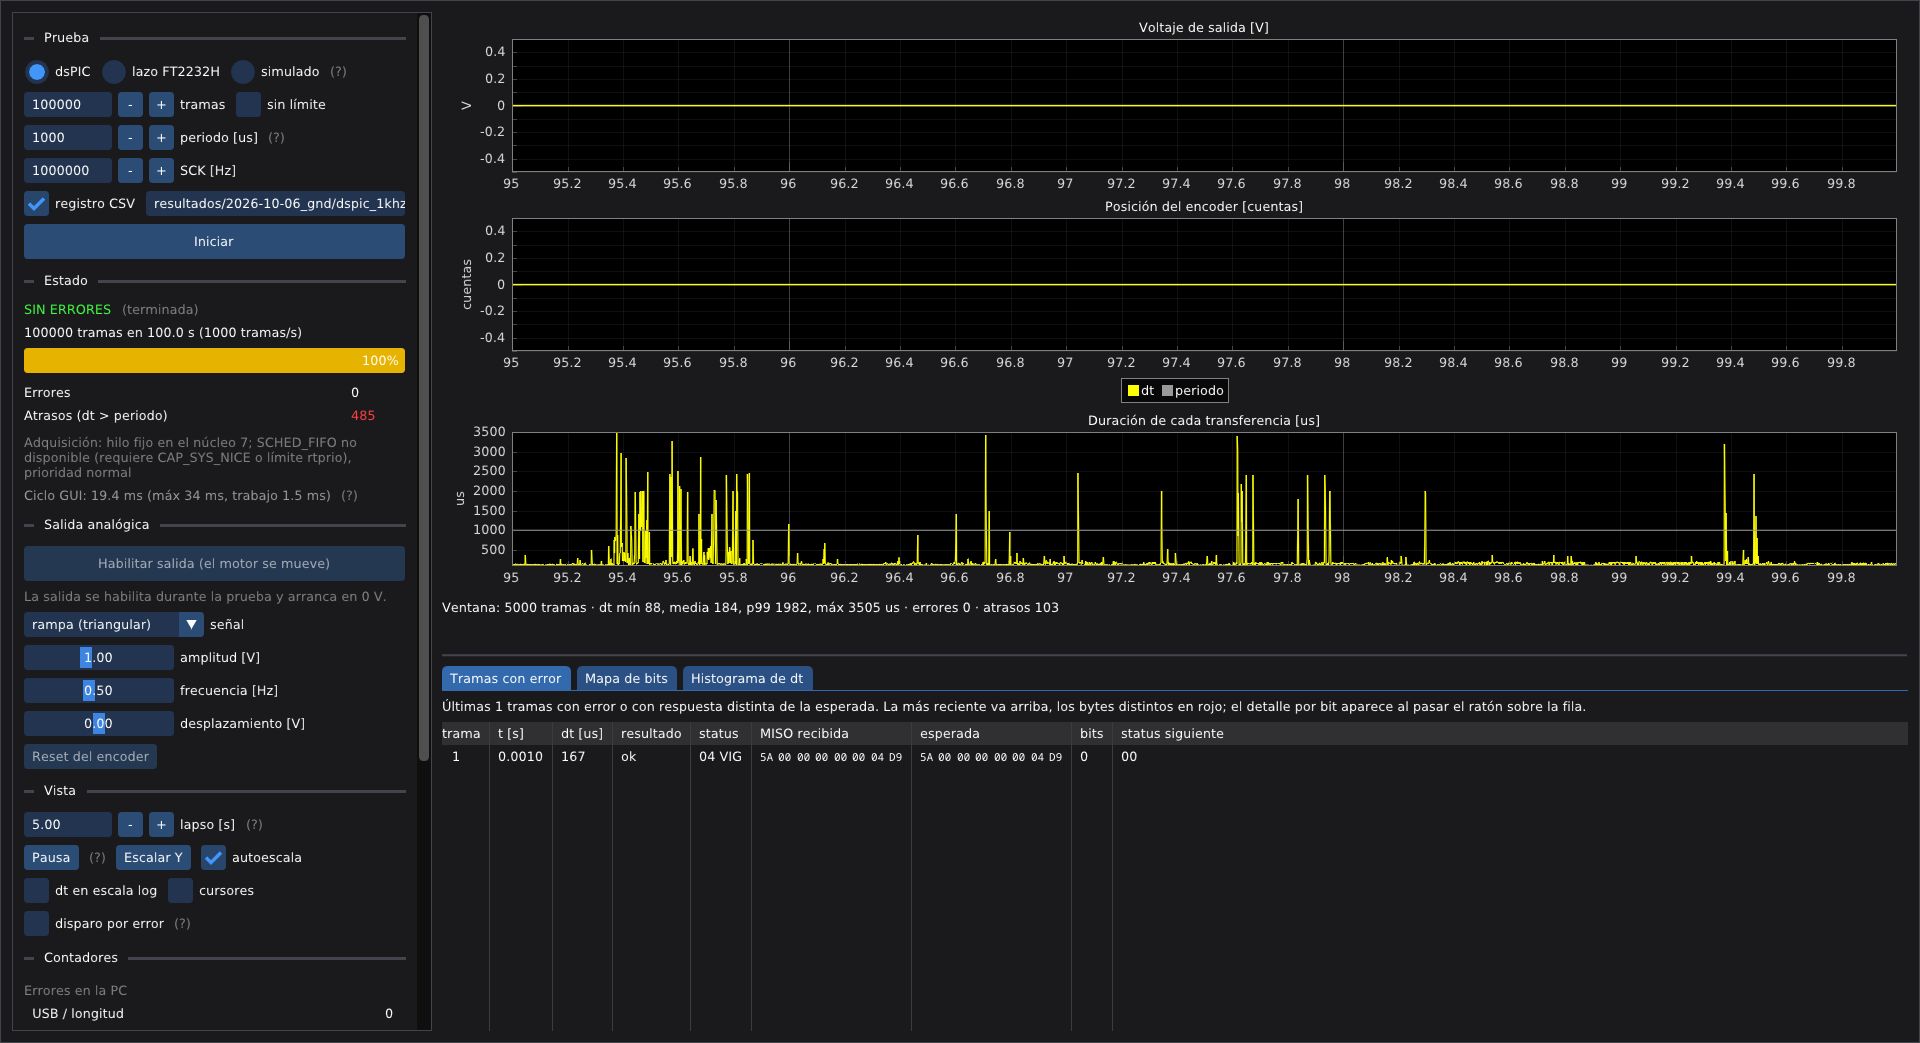
\includegraphics[width=\linewidth]{../resultados/2026-10-06_gnd/dspic_1khz.png}
\caption{Visor del enlace al terminar la prueba de 100\,000 tramas a 1\,kHz
con el cable de GND: cero errores.}
\label{fig:visor}
\end{figure}

% ===========================================================================
\section{Diagnóstico de los pulsos falsos en \code{CS}}
\label{sec:cs}

\subsection{Evidencia}

En la corrida con el visor y sin cable de GND, las respuestas dañadas no
contienen bits aislados erróneos, sino el inicio de la respuesta repetido a
mitad de la trama y recorrido algunos bits. La figura~\ref{fig:pulso}
presenta un caso.

\begin{figure}[H]
\centering
\resizebox{\linewidth}{!}{%
\begin{tikzpicture}[x=1cm, y=1cm]
  \node[rowlab] at (-0.3,3.3) {\code{CS}};
  \node[rowlab] at (-0.3,2.3) {MISO esperado};
  \node[rowlab] at (-0.3,1.3) {MISO recibido};
  \node[rowlab] at (-0.3,0.0) {dsPIC};

  % CS: baja al inicio, pulso falso durante el byte 1, sube al final
  \draw[semithick] (-0.2,3.6) -- (0,3.6) -- (0,3.0) -- (1.55,3.0) -- (1.55,3.6)
        -- (1.65,3.6) -- (1.65,3.0) -- (8.8,3.0) -- (8.8,3.6) -- (9.2,3.6);
  \node[font=\scriptsize, anchor=south] at (1.6,3.65) {pulso falso};

  \draw[densely dashed, black!50] (1.6,2.95) -- (1.6,0.95);
  \foreach \i/\t in {0/5A,1/AD,2/00,3/00,4/00,5/00,6/00,7/crc}
    \node[cell, fill=white] at (\i*1.1,2.0) {\t};
  \foreach \i/\t in {0/5A,5/00,6/00,7/00}
    \node[cell, fill=white] at (\i*1.1,1.0) {\t};
  \node[cell, fill=black!25] at (1.1,1.0) {B0};
  \foreach \i/\t in {2/05,3/AA,4/D0}
    \node[cell, fill=black!7] at (\i*1.1,1.0) {\t};

  \draw[semithick, fill=black!7] (0.1,-0.5) rectangle (3.9,0.5);
  \node[font=\scriptsize, align=center] at (2.0,0.0)
    {INT1: reinicia SPI1,\\arma la respuesta y el DMA};
  \draw[sig] (1.6,0.95) -- (1.6,0.5);
  \node[note, anchor=west, align=left] at (4.2,0.0)
    {la respuesta \code{5A AD \dots} vuelve a salir desde su inicio,\\
     recorrida 4 bits respecto a los bytes de la PC};
\end{tikzpicture}}
\caption{Respuesta dañada por un pulso falso en \code{CS}
(\code{resultados/2026-10-06\_dock/visor\_dspic\_1khz}). Se esperaba
\code{5A AD 00 00 00 00 00} y se recibió \code{5A B0 05 AA D0 00 00 00}: a
partir del byte~1 reaparecen \code{5A AD} desplazados medio byte.}
\label{fig:pulso}
\end{figure}

En otra respuesta, \code{5A 40 0B 4B 80 00 00 00} en lugar de
\code{5A 5C 00 \dots}, la secuencia de bits \code{01011010 01011100}
(\code{5A 5C}) aparece a partir del tercer bit del byte~1. De las 25
respuestas dañadas, la corrupción comienza en el byte~1 en 13, en el byte~2
en una y en el byte~7 en 11, según el momento en que ocurre el pulso; es el
mismo patrón observado en la campaña con puertos separados.

\subsection{Mecanismo}

El único código del firmware que vuelve a construir la respuesta desde su
inicio es la interrupción INT1, que se dispara con el flanco de subida de
\code{CS}. La secuencia es la siguiente:

\begin{enumerate}
\item Un pulso de ruido en \code{CS} se interpreta como fin de trama.
\item INT1 reinicia SPI1, construye la respuesta y rearma el DMA mientras la
  PC continúa la transferencia.
\item La PC recibe el resto de la respuesta desplazado algunos bits; el CRC
  no coincide.
\item Al subir \code{CS} al final de la transferencia, el dsPIC encuentra una
  trama incompleta y lo reporta con la bandera de longitud en la respuesta
  siguiente.
\end{enumerate}

Este mecanismo explica las dos observaciones que la hipótesis del DMA no
explicaba: que la falla dañe ambos sentidos a la vez y que la corrupción
comience en bytes concretos.

\subsection{Causa}

Las tarjetas no compartían una tierra directa: la única referencia común de
las señales del SPI era la tierra de los cables USB a través de la PC. Con
cada tarjeta en un puerto distinto, la diferencia de potencial y el ruido
entre ambas referencias eran suficientes para producir pulsos en \code{CS}
en el 0.7\,\% de las transferencias. El hub acortó el camino de retorno y
redujo la tasa a cero con \code{prueba\_enlace}, pero no con el visor, cuyo
uso de la GPU incrementa el ruido en la tierra de la PC. El cable de GND
eliminó los errores en todas las condiciones, lo que confirma la causa.

% ===========================================================================
\section{Cambios derivados}

\subsection{Vigilancia al inicio de una prueba}

Si el enlace permanece inactivo más de 50\,ms antes de una prueba, el dsPIC
reporta la bandera de vigilancia en la respuesta a la segunda trama. Ese
aviso es correcto, pero no corresponde a un error durante la prueba, y hacía
que la batería terminara con el resultado ``con errores'' sin que hubiera
ninguno. Se agregó la función \code{status\_contable()} en el núcleo común,
que omite esa bandera en la trama~1; la usan \code{prueba\_enlace}, el visor
y, con el mismo criterio, el generador de reportes. El registro CSV conserva
el \code{status} completo.

En \code{daqPic} ocurre lo mismo entre \code{mdlStart} y el primer paso de
simulación, intervalo en el que Simulink inicializa el resto del modelo y que
puede rebasar 50\,ms. El bloque ignora ahora la vigilancia en la respuesta del
segundo paso; sin este cambio, el indicador \code{Errores} comenzaría en~1 y
la prueba del paso~4 no podría cumplir el criterio de aceptación. El cambio
no se ha compilado, porque requiere MATLAB en Windows.

\subsection{Documentación}

\begin{itemize}
\item \code{README.md}: fila de GND en la tabla de conexiones y explicación
  del efecto de su ausencia.
\item \code{PRUEBAS.md}: el cable de GND como requisito; la fila ``pulsos
  falsos en \code{CS}'' en la tabla de interpretación de errores; la carga y
  la compilación del firmware en Linux; el punto~3 de la verificación con
  analizador lógico (entrega del segundo byte por el DMA) se marca como
  comprobado, ya que no hubo errores de secuencia en 200\,000 tramas.
\item Notas de análisis en cada carpeta de \code{resultados/}, incluidas en
  los reportes en PDF.
\end{itemize}

% ===========================================================================
\section{Salida analógica y conexión de la planta}

\subsection{Prueba de la rampa}

Se ejecutó el paso~3 del procedimiento con \code{prueba\_enlace -n 10000
-periodo 1000 -salida}: 10\,000 tramas a 1\,kHz con una rampa triangular de
$\pm1$\,V (códigos de 19\,660 a 45\,874) y la salida habilitada en todas las
tramas. La prueba terminó sin errores de comunicación y con la trama final de
0\,V. La posición del encoder permaneció en cero, como corresponde, ya que el
motor no estaba conectado. Falta observar \code{VOUTA} con osciloscopio.

\subsection{Niveles de la salida}

El DAC8554 sólo produce voltajes positivos:
\begin{equation*}
V_{\text{OUTA}} = V_{\text{REFL}} + \frac{\text{código}}{65536}\,
                  \left(V_{\text{REFH}} - V_{\text{REFL}}\right).
\end{equation*}
La escala del protocolo (13\,107 códigos por volt) corresponde a un intervalo
de 5\,V; con $V_{\text{REFL}} = 0$ y $V_{\text{REFH}} = 5$\,V, el ``0\,V''
del protocolo son 2.5\,V reales en la terminal~1 y la rampa de $\pm1$\,V
debe observarse entre 1.5 y 3.5\,V, con periodo de 2\,s. La
tabla~\ref{tab:dac} indica las terminales del adaptador PA0017C, que
conserva la numeración del circuito.

\begin{table}[H]
\centering
\small
\begin{tabular}{@{}cll|cll@{}}
\toprule
Term. & Nombre & Conexión & Term. & Nombre & Conexión \\
\midrule
1 & VOUTA & etapa de potencia & 16 & LDAC & GND \\
2 & VOUTB & sin uso & 15 & ENABLE & GND \\
3 & VREFH & 5\,V & 14 & A1 & GND \\
4 & AVDD & alimentación & 13 & A0 & GND \\
5 & VREFL & GND & 12 & IOVDD & alimentación \\
6 & GND & GND & 11 & DIN & RB2 \\
7 & VOUTC & sin uso & 10 & SCLK & RB0 \\
8 & VOUTD & sin uso & 9 & SYNC & RB4 \\
\bottomrule
\end{tabular}
\caption{Terminales del DAC8554 y conexión esperada según el firmware.
Fuente de la distribución: hoja de datos SLAS431B de Texas Instruments.}
\label{tab:dac}
\end{table}

\subsection{Motor y encoder}

El motorreductor Pittman GM8724S017-R1 es de 14\,V con escobillas. Su
encoder de 500 ciclos por revolución produce, con el conteo en cuadratura
del QEI, 2000 cuentas por revolución del motor. Para su conexión se
consideran los puntos siguientes:

\begin{itemize}
\item \textbf{Etapa de potencia.} El DAC no puede alimentar el motor. Se
  requiere un amplificador con entrada analógica que reste el nivel de
  2.5\,V y entregue una tensión bipolar de hasta $\pm14$\,V con la corriente
  del motor; un puente H con entrada PWM no es adecuado sin una etapa
  adicional. La etapa de potencia aparece como ``por confirmar'' en la
  arquitectura y debe identificarse.
\item \textbf{Encoder.} En otros encoders Pittman de 500 CPR el conector de
  cinco terminales es: 1~GND, 2~índice, 3~canal~A, 4~+5\,V, 5~canal~B. Este
  dato no se ha confirmado para el modelo instalado. El encoder requiere
  5\,V; los canales A y B se conectan a RB8 y RB9.
\item \textbf{Niveles lógicos.} RB8 y RB9 comparten función con entradas
  analógicas (AN10, AN11) y con la programación (PGD1, PGC1). Mientras no se
  confirme en la hoja de datos que toleran 5\,V, se recomienda un divisor
  (2.2\,k$\Omega$ en serie y 3.3\,k$\Omega$ a GND) en cada canal.
\end{itemize}

% ===========================================================================
\section{Trabajo pendiente y recomendaciones}

\begin{enumerate}
\item Observar \code{VOUTA} con osciloscopio durante la rampa del paso~3.
\item Identificar la etapa de potencia del motor y verificar que compense el
  nivel de 2.5\,V antes de conectar el motor.
\item Confirmar la distribución del conector del encoder y los niveles
  admisibles en RB8 y RB9; probar el encoder girando el eje a mano con el
  visor.
\item Compilar \code{daqPic} en Windows, ejecutar el modelo de prueba y
  verificar que \code{Errores} y \code{Atrasos} terminen en cero.
\item Repetir la medición de tiempos en Windows con la PC sin carga
  adicional, para fijar el periodo de muestreo mínimo.
\item Medir con analizador lógico la duración de la interrupción de fin de
  trama en RD10.
\item Opcional: rechazar en INT1 los flancos en que \code{CS} ya volvió a
  nivel bajo, como protección adicional en caso de que el cable de GND se
  desconecte. No es necesario con la conexión actual.
\item Realizar la prueba en contra con las tarjetas en puertos separados y
  el cable de GND, para documentar que la conexión USB deja de influir.
\end{enumerate}

% ===========================================================================
\appendix
\section{Historial de cambios}

\begin{longtable}{@{}llp{10.2cm}@{}}
\toprule
Fecha & Commit & Descripción \\
\midrule
\endhead
2026-10-01 & \code{b0176e2} & Propuesta de solución al problema de concurrencia SPI y diagrama de arquitectura. \\
2026-10-02 & \code{fae8880} & Documentación del DAC8554 y redacción del README. \\
2026-10-02 & \code{a89bc2e} & Protocolo full-duplex, firmware \code{dsPicDaq} con DMA, \code{prueba\_enlace}, S-Function \code{daqPic} y procedimiento de pruebas. \\
2026-10-03 & \code{7e7edd1} & Conversión de voltaje a código centralizada en el protocolo. \\
2026-10-03 & \code{d4d7719} & Modelo de la vigilancia y ampliación de las pruebas del protocolo. \\
2026-10-03 & \code{47ca3fd} & Integración continua con gcc y clang. \\
2026-10-05 & \code{2b8c056} & \code{prueba\_enlace} en Linux con libftdi1 y lazo interno. \\
2026-10-05 & \code{4c9e9ea} & Registro por trama, reportes en PDF y primeras pruebas con la tarjeta. \\
2026-10-05 & \code{391c072} & PLL ($F_{cy} = 50$\,MHz) y reporte de la causa de reinicio. \\
2026-10-05 & \code{0f01466} & Visor en tiempo real y batería de pruebas. \\
2026-10-05 & \code{3099948} & Resultados con PLL y con el visor. \\
2026-10-06 & \code{8cdfc55} & Resultados con ambas tarjetas en un hub. \\
2026-10-06 & \code{1b8b3d2} & Cable de GND, diagnóstico de los pulsos en \code{CS} y vigilancia inicial. \\
\bottomrule
\end{longtable}

\section{Ubicación de los resultados}

\begin{table}[H]
\centering
\small
\begin{tabularx}{\linewidth}{@{}lX@{}}
\toprule
Carpeta & Contenido \\
\midrule
\code{resultados/2026-10-05} & $F_{cy} = 4$\,MHz; incluye SCK de 250 y 500\,kHz \\
\code{resultados/2026-10-05\_pll} & PLL, puertos separados, \code{prueba\_enlace} \\
\code{resultados/2026-10-05\_visor} & PLL, puertos separados, visor \\
\code{resultados/2026-10-06\_dock} & PLL, un hub, \code{prueba\_enlace}; corrida del visor sin GND \\
\code{resultados/2026-10-06\_gnd} & PLL, un hub, cable de GND, visor \\
\code{resultados/2026-10-06\_salida} & Rampa de $\pm1$\,V (paso~3) \\
\bottomrule
\end{tabularx}
\end{table}

Cada carpeta contiene, por prueba, la salida del programa (\code{.txt}), el
reporte (\code{.pdf}) y, cuando existen, las notas de análisis
(\code{\_notas.tex}) y la captura del visor (\code{.png}).

\end{document}
